\documentclass[a4paper]{article}

\usepackage[czech]{babel} %https://github.com/michal-h21/biblatex-iso690
\usepackage[
   backend=biber      % if we want unicode 
  ,style=iso-numeric % or iso-numeric for numeric citation method          
  ,babel=other        % to support multiple languages in bibliography
  ,sortlocale=cs_CZ   % locale of main language, it is for sorting
  ,bibencoding=UTF8   % this is necessary only if bibliography file is in different encoding than main document
]{biblatex}

\usepackage[utf8]{inputenc}
\usepackage{fancyhdr}
\usepackage{amsmath}
\usepackage{amssymb}
\usepackage[left=2cm,right=2cm,top=2.5cm,bottom=2.5cm]{geometry}
\usepackage{graphicx}
\usepackage{pdfpages}
\usepackage{url}
\usepackage{subcaption}

\usepackage{siunitx}
\sisetup{locale = DE}  %, separate-uncertainty = true    kdybych chtel +/-

\usepackage{float}
\newfloat{graph}{htbp}{grp}
\floatname{graph}{Graf}
\newfloat{tabulka}{htbp}{tbl}
\floatname{tabulka}{Tabulka}

\renewcommand{\thefootnote}{\roman{footnote}}

\pagestyle{fancy}
\lhead{Praktikum III - (16) Měření indexu lomu Fraunhoferovou metodou}
\rhead{Vladislav Wohlrath}
\author{Vladislav Wohlrath}

\bibliography{source}

\newcommand{\uhel}[3]{\ang{#1 ; #2 ; #3}}

\begin{document}

\begin{titlepage}
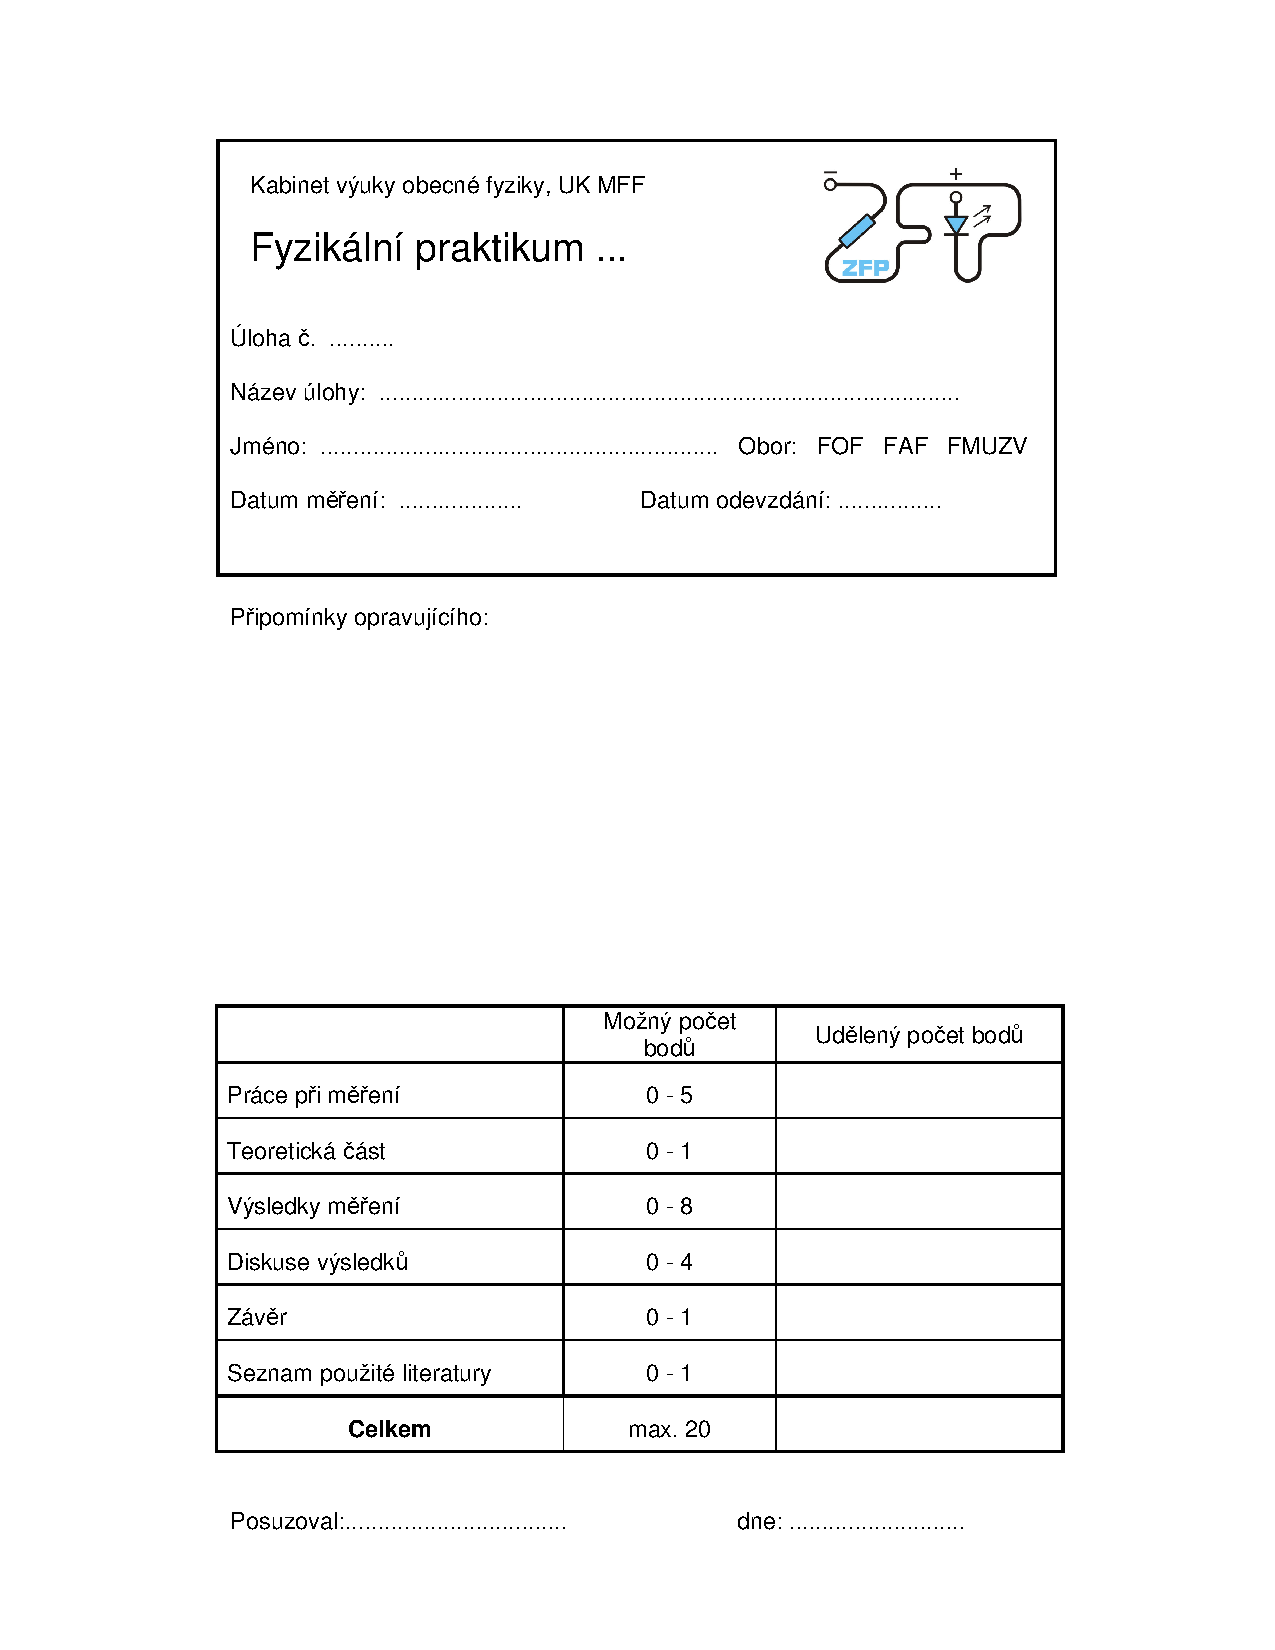
\includepdf[pages={1}]{./graficos/titlelist.pdf}
\end{titlepage}

\section*{Pracovní úkoly}
\begin{enumerate}
\item Seřiďte goniometr.
\item Změřte lámavý úhel skleněného hranolu a proměřte indexy lomu čar spektra rtuťové výbojky.
\item Změřte lámavý úhel kyvety a proměřte pro přiloženou kapalinu indexy lomu čar spektra rtuťové výbojky.
\item Naměřené hodnoty zpracujte graficky do disperzních křivek. Vypočtěte střední disperzi, relativní disperzi a Abbeovo číslo pro změřené materiály.
\item Odvoďte výraz pro chybu nepřímého měření indexu lomu. Spočtěte její velikost a diskutujte, kolik desetinných míst indexu lomu tato metoda zaručuje.

\end{enumerate}

%Teoretická část
\section*{Teoretická část}

%Výsledky měření
\section*{Výsledky měření}

%Diskuze výsledků
\section*{Diskuze}
V grafech \ref{g:h} a \ref{g:k} jsme závislost fitovali funkcí tvaru \cite{skripta}
\begin{equation*}
n(\lambda) = n_0 + \frac{a}{\lambda + \lambda_0} \,.
\end{equation*}
Pro hranol jsme použili parametry
\begin{equation*}
n_0=1,49 \qquad \qquad a=\SI{10.4}{\per\nm} \qquad \qquad \lambda_0=\SI{-108}{\nm}
\end{equation*}
pro kapalinu pak
\begin{equation*}
n_0=1,32 \qquad \qquad a=\SI{6.6}{\per\nm} \qquad \qquad \lambda_0=\SI{-130}{\nm} \,.
\end{equation*}
Podle grafu tato funkce závislost dobře aproximuje.


Nejsme si vědomi žádné systematické chyby, které bychom se dopustili. Systematická chyba způsobená nepřesným odečítáním ze stupnice goniometru působila při měření ve druhém směru opačně, takže se vyrušila.

Měření považujeme za velice přesné a hodnotami indexů lomů jsme si skutečně jisti na tři číslice za desetinnou čárkou.

Při výpočtu střední disperze, relativní disperze a Abbeova čísla se odečítají blízké hodnoty, což má za následek vysokou relativní chybu. Díky přesnosti měření indexu lomu je však i tato chyba rozumná.



%Závěr
\section*{Závěr}


\printbibliography[title={Seznam použité literatury}]

\end{document}